\documentclass[tikz,border=8pt]{standalone}
% Shared look for every TikZ diagram. Load with \input{../../tools/tikz-style.tex}
\usepackage[T1]{fontenc}
\usepackage{lmodern}
\renewcommand{\sfdefault}{lmr}  % diagrams use the same serif as the text
\usetikzlibrary{arrows.meta, positioning, shapes.geometric, calc, fit, backgrounds}
\definecolor{cblue}{HTML}{4C78A8}
\definecolor{corange}{HTML}{F58518}
\definecolor{cgreen}{HTML}{54A24B}
\definecolor{cred}{HTML}{E45756}
\definecolor{cpurple}{HTML}{B279A2}
\definecolor{cgrey}{HTML}{6B6B6B}
\tikzset{
  every picture/.style={font=\sffamily, line width=1.2pt},
  box/.style={draw=#1, fill=#1!12, rounded corners=4pt, align=center, inner sep=7pt, minimum height=1.1cm},
  box/.default=cgrey,
  arrow/.style={-{Stealth[length=3mm]}, draw=cgrey, line width=1.4pt},
  title/.style={font=\sffamily\bfseries\Large},
  note/.style={font=\sffamily\small, text=cgrey, align=center},
}
\AtBeginDocument{\hyphenpenalty=10000 \exhyphenpenalty=10000}

\begin{document}
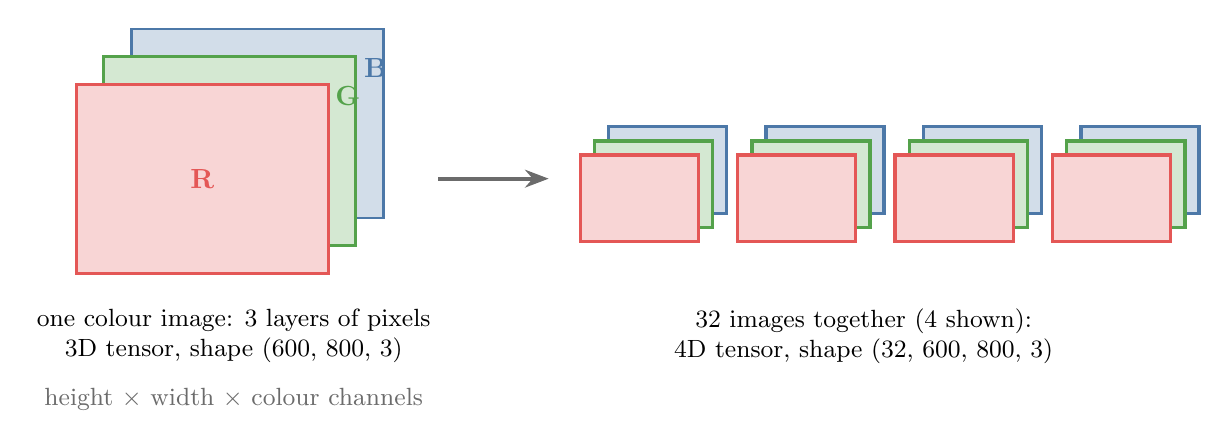
\begin{tikzpicture}
  % one colour image = 3 channel layers
  \foreach \ch/\c [count=\i] in {B/cblue, G/cgreen, R/cred}
    \filldraw[draw=\c, fill=\c!25, line width=1pt] ({(3-\i)*0.35},{(3-\i)*0.35}) rectangle ++(3.2,2.4);
  \node[cred, font=\bfseries] at (1.6,1.2) {R};
  \node[cgreen, font=\bfseries] at (3.45,2.25) {G};
  \node[cblue, font=\bfseries] at (3.8,2.6) {B};
  \node[align=center, font=\small] at (2.0,-0.8) {one colour image: 3 layers of pixels\\3D tensor, shape (600, 800, 3)};
  \node[note] at (2.0,-1.6) {height $\times$ width $\times$ colour channels};
  % a batch of images
  \draw[arrow] (4.6,1.2) -- (6.0,1.2);
  \foreach \k in {0,...,3} \foreach \ch/\c [count=\i] in {B/cblue, G/cgreen, R/cred}
    \filldraw[draw=\c, fill=\c!25] ({6.4+\k*2.0+(3-\i)*0.18},{0.4+(3-\i)*0.18}) rectangle ++(1.5,1.1);
  \node[align=center, font=\small] at (10.0,-0.8) {32 images together (4 shown):\\4D tensor, shape (32, 600, 800, 3)};
\end{tikzpicture}
\end{document}
